\subsection{Background}

% Machine Learning (ML) has gained an increased interest from game researchers, achieving remarkable success on training AI agents for very popular games, such as AlphaStar on Starcraft 2 \citeptenth{p10alphastarblog} and OpenAI Five on Dota 2 \citeptenth{p10berner2019dota}. 

% Here playing modeling in general
Player modeling, the ability to recognize general socio-emotional and cognitive/behavioral patterns in players~\citeptenth{p10thawonmas2019artificial}, has been appointed by the game research community as an essential process in many aspects of game development, such as designing of new game features, driving marketing and profitability analyses, or as a means to improve PCG and game content adaptation. Player modeling frequently relies on data-driven and ML approaches to create such models from user data or user-generated gameplay data~\citeptenth{p10melhart2020feel,p10Melhart2019-ModellingMotivation,p10canossa2015towards,p10Holmgard2019-proceduralPersonas}. 

Modeling users and players can have different goals and use multimodal data. User data can be used to understand and enable behavior for agents in games. For instance, Melhart et al. model a user's \textit{Theory of Mind}, finding that players' perception of an agent's frustration is more a cognitive process than an affective response~\citeptenth{p10melhart2020feel}. Alvarez and Vozaru explored personality-driven agents, evaluating how observers judged and perceived agents using their personality data from their personality tests when encountering multiple situations~\citeptenth{p10Alvoz2019-PersonalityDriven}. Gameplay data can show player behavior, as well as help developers understand their player base. Melhart et al. used gameplay data from \textit{Tom Clancy's The Division} to find predictors of player motivation~\citeptenth{p10Melhart2019-ModellingMotivation}, and Drachen and Canossa used playing behavior data from \textit{Tomb Raider Underworld} and identified four types of players as behavior clusters, which provide relevant information for game testing and mechanic design \citeptenth{p10Drachen2009-playerModellingTombRaider}.

Furthermore, the combination of Machine Learning (ML) with PCG has led to the rise of Procedural Content Generation via Machine Learning (PCGML), defined as the generation of game content by models that have been trained on existing game content \citeptenth{p10summerville2018procedural}. PCGML has been used for autonomous content generation, content repair, content critique, mixed-initiative design, or content adaptation. A promising PCGML usage is in the area of content adaptation, where using player and user models are essential to adapt the generated content~\citeptenth{p10Duque2021-BayesianbasedPlayerModel,p10togelius2007-AutomaticPersonalisedRaceGames,p10Yannakakis2011-experiencedrivenPCG}. 

Content adaptation can take place as players play or use the content online or offline, building models from collected data. For instance, Duque et al. adapt and adjust the difficulty of generated content as players play the game using bayesian optimization~\citeptenth{p10Duque2021-BayesianbasedPlayerModel}. Summerville et al. model players automatically and implicitly by learning from video traces; generating levels that correspond to the latent player models~\citeptenth{p10Summerville2016-LearningPlayerTailoredPlatformer}. Player models can also be used to enhance and adapt design tools, specifically MI-CC tools. Migkotzidis and Liapis use player models as surrogate models to generate content assisting game designers in the creation of more relevant content for specific players~\citeptenth{p10Panagiotis2021-susketch}. Similarly, Holmgård et al. use player personas based on player archetypes as content critics to help designers adapt their content to different archetypes~\citeptenth{p10Holmgard2019-proceduralPersonas}. Their work on player personas is similar to our proposed work, yet instead of personas based on player archetypes, we propose personas based on design style.

% modeling using video traces, use video traces to generate content, and simultaneously model the players implicitly by learning a latent model of the player in the videos automatically model players

% Duque et al. proposed the use of bayesian optimization to adjust and personalise the difficulty of generated content to users based on their performance~\citeptenth{p10Duque2021-BayesianbasedPlayerModel}. 

% Duque et al. adapt and adjust the difficulty of generated content as players play the game using bayesian optimization~\citeptenth{p10Duque2021-BayesianbasedPlayerModel}. Similarly, Summerville et al. 




% Usually, content is adapted by constructing some player model and then using that model to generate content in an off-line fashion 




% , which depending on the goal, would adapt the content one way or another.



% Depending on the goal of what should be adapted

% Depending on the goal of what should be adapted 

% Content adaptation can take many forms depending on the goals, one can adapt the difficulty 



% Content can be adapted to fulfill different goals. For instance, it 

% Adapting generated content requires 

% Adapting content requires 

% Content adaptation can use different types of data and be used to adapt content 

% Content adaptation uses somehas many uses and can be used to 

% Collective data, as opposed to single-user user data, helps mitigating lack of data used to train these models and to show trends and in our case, archetypes. 




% , adjusting and personalising difficulty based on an specific goal 

% Perhaps Duque can come in here!

% % Similarly, \citeptenth{p10guzdial2016game} clusters Super Mario Bros. level design chunks out of gameplay video, and then builds a probabilistic model over these to generate new levels. 

% Reviewer 2 wants this paper in: Summerville et al.~\citeptenth{p10Summerville2016-LearningPlayerTailoredPlatformer}.

% \citeptenth{p10Holmgard2019-proceduralPersonas} Here we talk about this in relation to:





% Melhart et al. used gameplay data from \textit{Tom Clancy's The Division} to find predictors of player motivation, which helpt them understand psychological effecs of gameplay~\citeptenth{p10Melhart2019-ModellingMotivation}, and Drachen and Canossa used playing behavior data from \textit{Tomb Raider Underworld} 

% Modeling players can use multimodal data to achieve its goal

% Modeling players can take different forms and applications, and use multimodal data to achieve 

% Moreover, training models on gameplay data from \textit{Tom Clancy's The Division} has also been used to model, and therefore find predictors of player motivation \citeptenth{p10Melhart2019-ModellingMotivation}, which renders a very valuable tool for understanding the psychological effects of gameplay. Former research followed a similar approach in \textit{Tomb Raider Underworld}, training player models on high-level playing behavior data, identifying four types of players as behavior clusters, which provide relevant information for game testing and mechanic design \citeptenth{p10Drachen2009-playerModellingTombRaider}. Melhart et al. take these approaches one step further by modeling a user's \textit{Theory of Mind} in a human-game agent scenario \citeptenth{p10melhart2020feel}, finding that players' perception of an agent's frustration is more a cognitive process than an affective response. 
% Furthermore, Alvarez and Vozaru explored personality-driven agents based on individuals' personalities using the \textit{cybernetic big five model}, evaluating how observers judged and perceived agents using data from their personality test when encountering multiple situations~\citeptenth{p10Alvoz2019-PersonalityDriven}.

% % Here Player modeling for content adaptation




% experience~\citeptenth{p10togelius2007-AutomaticPersonalisedRaceGames,Yannakakis2011-experiencedrivenPCG}, 

% where user models can be created and used for adapting content based on a serie 
% Content adaptation while possible and promising, 

% with applications to autonomous content generation, content repair, content critique, data compression, and mixed-initiative design. Player modeling, the ability to recognize general socio-emotional and cognitive/behavioral patterns in players~\citeptenth{p10thawonmas2019artificial}, has been appointed by the game research community as an essential process in many aspects of game development, such as designing of new game features, driving marketing and profitability analyses, or as a means to improve PCG and game content adaptation. 


% Player modeling frequently relies on data-driven and ML approaches to create such models out of several sorts of user-generated gameplay data \citeptenth{p10liapismodellingquality19,melhart2020feel,canossa2015towards,Holmgard2019-proceduralPersonas,Melhart2019-ModellingMotivation}.

% Using player data from \textit{Iconoscope}, a freeform creation game for visually depicting semantic concepts, Liapis et al. trained and compared several ML algorithms by their ability to predict the appeal of an icon from its visual appearance~\citeptenth{p10liapismodellingquality19}.  Scheherezade \citeptenth{p10li2013story} presents a data-driven approach to story generation by building models for specific topics from a corpus of narrative examples, whose generated spaces are later sampled to generate stories. 

% Collective data, as opposed to single-user user data, helps mitigating lack of data used to train these models and to show trends and in our case, archetypes. 



%  using Bartle's player archetypes~\citeptenth{p10bartle1996-taxonomy}

%Alvarez and Vozaru did similar work, exploring personality-driven agents based on individuals' personality using the \textit{cibernetic big five model}, evaluating how observers judged and perceived agents using data from their personality test when encountering multiple situations~\citeptenth{p10Alvoz2019-PersonalityDriven}.

%Alvarez and Vozaru did similar work, exploring personality-driven agents based on individuals' personality using the \textit{cibernetic big five model}, which treats personality-driven agents as goal-based entitites, evaluating how observers judged and perceived agents using data from their personality test when encountering multiple situations~\citeptenth{p10Alvoz2019-PersonalityDriven}.
%modeling individual agents based 

\subsubsection{Designer-centric Perspective}

Mixed-initiative co-creativity (MI-CC)~\citeptenth{p10yannakakis2014micc}, is the subset of PCG algorithms where human users and AI systems engage in a constant mutual inspiration loop towards the creation of game content \citeptenth{p10charity2020baba,p10machado2019pitako,p10shaker2013ropossum,p10smith_tanagra:_2011,p10liapis_generating_2013}. Understanding the designer's behavior and experience, as well as predicting their intentions is key for mixed-initiative creative tools while aiming to offer in real-time user-tailored procedurally generated content. 

While player modeling is key for generating content adapted to players, adapting tools, systems, and AI methods for designing games requires a shift towards a designer-centric perspective, focusing on Designer Modeling. \emph{Designer Modeling}, akin to player modeling, refers to the creation of models of either individual designers or groups of designers informed by how they create various types of content. Liapis et al.~\citeptenth{p10Liapis2013-designerModel,p10Liapis2014-designerModelImpl} introduced designer modeling for personalized experiences when using computer-aided design tools, with a focus on the integration of such in automatized and mixed-initiative content creation. The focus is on capturing the designer's style, preferences, goals, intentions, and iterative design process to create representative models of designers.



% to create personalized experiences and adapted tools. Liapis et al. described designer modeling as capturing the style, process, preferences, intentions, and goals of designers as they create content~\citeptenth{p10Liapis2013-designerModel}. Furthermore, Liapis et al. implemented a prototype of such model in the Sentient Sketchbook~\citeptenth{p10Liapis2014-designerModelImpl}, where the focus was on using the designer's current design and choice-based evolution to capture process, style, and goals. Alvarez and Font~\citeptenth{p10Alvarez2020-DesignerPreference}, proposed the use of the behavior characteristics of the generated levels where a neural network was trained on the estimated preference of the designer using a similar approach as the choice-based evolution from Liapis et al.~\citeptenth{p10Liapis2014-designerModelImpl}.

% adapting tools, systems, and AI methods 

% A paradigm that seeks to combine 



EXplainable AI (XAI) is an emergent research field that holds substantial promise for improving model explainability while maintaining high-performance levels~\citeptenth{p10adadi2018peeking,p10Doshi-Velez2018}. Explanations should be aligned with the users' understanding to not hinder the usability of systems, as demonstrated by Nourani et al.~\citeptenth{p10Nourani2019-meaningfulExplanations}, who discuss the effects of meaningful and meaningless explanations to users of an AI interactive systems.

Zhu et al.~\citeptenth{p10Zhu2018-XAIDesignersMICC} proposed the field of eXplainable AI for Designers (XAID) as a human-centered perspective on MI-CC tools. This work discusses three principles of mixed-initiative, \emph{explainability}, \emph{initiative}, and \emph{domain overlap}, where the latter focuses on the study of the overlapping creative tasks between game designers and black-box PCG systems in mixed-initiative contexts. This work deems of high relevance the inclusion of data-driven and trained artifacts to facilitate a fluent bi-directional communication of the internal mechanisms of such a complex co-creative process in which \textit{the designer provides the vision, the AI provides capabilities, and they merge that into the creation}. Mapping the designer's internal model to the AI's internal model is suggested as a meaningful way for creating a common ground that establishes a shared language that enables such communication. Our method, and designer modeling in general, aims to develop this designer's internal model to enhance MI-CC tools by adapting the AI's functionality towards designers' needs and aligning to their objectives.

% Recent research proposes visualization techniques based on game design patterns \citeptenth{p10guzdial2018explainable} and interactive level designer tools \citeptenth{p10xie2019interactive}, aiming to explain machine learning principles to game designers. 

% Our work  aims at developing these designer's models 

% of designers and align 



Moreover, Guzdial et al.'s~\citeptenth{p10guzdial-lvldsg-aiide-2018} discuss the insufficiency of current approaches to PCGML for MI-CC, as well as the need for training on specific datasets of co-creative level design. Guzdial et al. work on the mixed-initiative Morai Maker~\citeptenth{p10guzdial2019friend} shows the relevance of exploring the ways designers and AI interact towards co-creation, identifying four human-AI relationships (friend, collaborator, student, and manager), as well as the different ways they impact on the designer-user experience. Our study advocates for the importance of designer modeling through ML as the generation of surrogate models of designer styles by training on existing designer-generated data, aiming for an improvement in quality and diversity in computational creativity and, in particular, MI-CC tools. 

% Nevertheless, the player is the designer in MI-CC, and gameplay data is replaced by a compilation of designer-user actions and AI model reactions over time while both user and model are engaged in a mutually inspired creative process.

% A fluent MI-CC loop should provide good human understanding and interpretation of the system, as well as accurate user behavior modelling by the system, capable of projecting the user's subsequent design decisions \citeptenth{p10ComptonPhD}. 

%Similar to user or player modeling, designer modeling for content creation tools (CAD and MI-CC tools) was suggested by Liapis et al~\citeptenth{p10Liapis2013-designerModel}, where it is proposed the use of designers models that capture their styles, preferences, goals, intentions, and interaction processes. In their work, they suggest methods, indications, and advice on how each part can be model to be integrated into a holistic designer model, and how each game facet can use and benefit from designer modeling. Moreover, in \citeptenth{p10Liapis2014-designerModelImpl} the same authors discuss their implementation of designer modeling and the challenges of integrating all together in their MI-CC tool, Sentient Sketchbook, which had a positive outcome on the adaptation of the tool towards individual “artificial” users.

% Shifting towards a designer-centric perspective means that besides focusing on player modeling, it is necessary to focus on modeling the designers. Liapis et al.~\citeptenth{p10Liapis2013-designerModel,Liapis2014-designerModelImpl} introduced designer modeling for personalized experiences when using computer-aided design tools, with a focus on the integration of such in automatized and mixed-initiative content creation. The focus is on capturing the designer's style, preferences, goals, intentions, and iterative design process to create representative models of designers.

% Through these models, designer's and their design process could be understood in-depth, enabling adaptive experiences, further reducing their workload and fostering their creativity. 

%\citeptenth{p10charity2020baba,machado2019pitako,shaker2013ropossum,smith_tanagra:_2011,Machado2017,liapis_generating_2013}. 

% Moreover, goal 13 in the guidelines for Human-AI interaction \citeptenth{p10amershi2019guidelines} highlights the importance of learning from user behavior and personalize the user’s experience by learning from their actions over time. 


%Nourani et al.~\citeptenth{p10Nourani2019-meaningfulExplanations}, who discuss the effects of meaningful and meaningless explanations to users of an AI interactive systems, and their results demonstrates that when an explanation is not aligned with human-logic it significantly affect the user's perception of the system and it's usability is hindered.

% One of the aims with MI-CC is the true and proactive collaborative creation and design between humans and AI. However, to establish  

% However, for this interaction to be fully fleshed, the human needs to understand the behavior of the AI through interpretable and explainable models and systems, and the AI needs to recognize and interpret the intentions of the humans seamlessly as they create their designs. The former is the focus of~\emph{Interpretable and Explainable AI}, which seek to create or adapt models and systems for a better workflow between humans and AI, where humans can understand the AI's decision process to enable trust relationships and reach deeper interactions~\citeptenth{p10Zhu2018-XAIDesignersMICC,Doshi-Velez2018,adadi2018peeking}. The latter, which is the focus of this paper, would mean that the AI could adapt its behavior and functionality to the needs, expertise, and workflow of individual designers or specific group of designers. To do so, the AI is required to do an analysis on several design processes such as the designer's preferences, styles, and goals, which holistically is called \emph{Designer Modeling}~\citeptenth{p10Liapis2013-designerModel,Liapis2014-designerModelImpl}.



\subsubsection{The Designer Preference Model in EDD}

EDD is an MI-CC tool where designers can create dungeons and rooms; meanwhile, a PCG system analyzes their design and proposes suggestions to the designer~\citeptenth{p10Alvarez2018,p10Baldwin2017}. EDD uses \emph{Interactive Constrained MAP-Elites} (IC MAP-Elites)~\citeptenth{p10alvarez2019empowering}, an evolutionary algorithm that combines Constrained MAP-Elites~\citeptenth{p10Khalifa2018} with interactive and continuous evolution. 

The work presented in \citeptenth{p10Alvarez2020-DesignerPreference} introduced the Designer Preference Model, a data-driven solution that learns from user-generated data based on their choices while using EDD. Both systems constantly interact and depend on each other, so that the Designer Preference Model learns from the selected suggestions, and IC MAP-Elites uses the Designer Preference Model as a designer's surrogate model to complement the fitness evaluation of new individuals. The results showed the need for stability and robustness in the data-driven model, to counterbalance the highly dynamic designer's creative process.  

% This approach's main goal is modeling the user's design style to better assess the tool's generated content, increasing the user's agency over the generated content without stalling the MI-CC loop \citeptenth{p10ComptonPhD} or decreasing user fatigue with periodical suggestion handpicking \citeptenth{p10liapis2016mixed,Takagi2001-InteractiveEvo}. The results showed the need for stability and robustness in the data-driven model, to counterbalance the highly dynamic designer's creative process. 

\begin{figure*}[t!]
\centerline{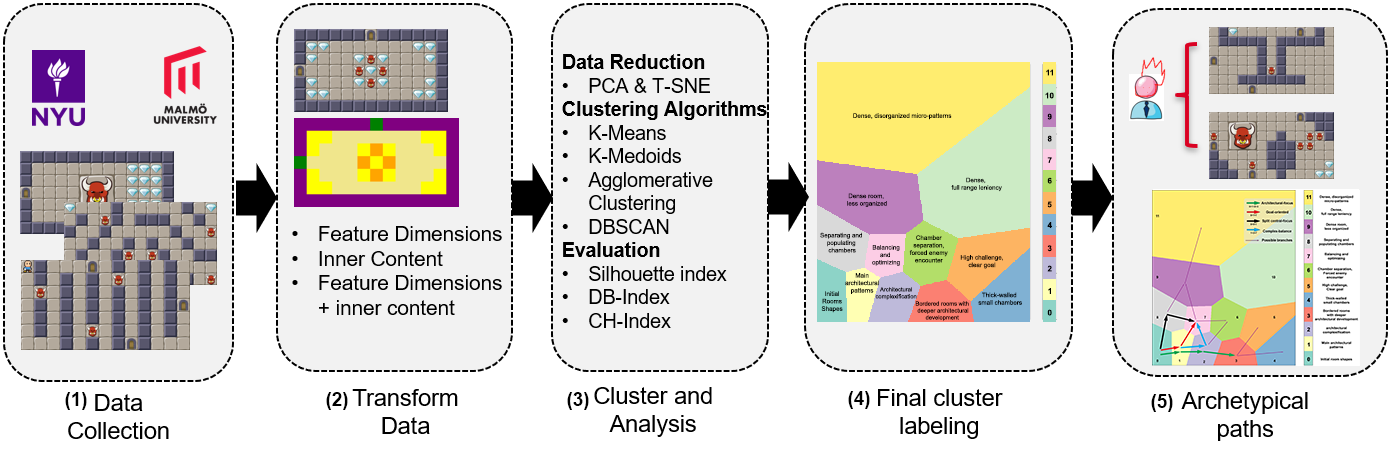
\includegraphics[width=\textwidth]{figures/figure1.png}}
\caption{The stages of the design style clustering development: (1) Data was first collected through two user studies. (2) Then, using the design sequences, the data was processed into five different datasets, one using the room images, a second using the tiles information, and three using tabular information. (3) A data reduction technique was applied to different datasets, and then they were clustered and internally evaluated. (4) The clusters were formed, picked from the best performing methods, and labeled based on the data points within each cluster. The clusters were evaluated by visualizing how a typical design session traverse the various clusters, and K-Means (K=12) was chosen as the final approach. (5) Finally, using this final approach all the sequences were clustered and archetypical paths were identified.%(5) The final approach,  K-Means (K=12) was evaluated by visualizing how a typical design session traverse the various clusters. Finally, the sequences were clustered by the final approach and archetypical paths were identified.
} \label{fig:approach-steps}
\end{figure*}